\documentclass[a4paper]{book}
\usepackage[utf8]{inputenc}                                      
\usepackage[OT4]{fontenc}  
\usepackage[polish]{babel} 
\usepackage{indentfirst}
\usepackage{graphicx} 
\usepackage{hyperref}
% potrzebny jeżeli korzystamy z listingów
\usepackage{color}
\usepackage{listings}
\usepackage{array}
\usepackage{makecell}
\renewcommand\theadalign{bc}
\renewcommand\theadfont{\bfseries}
\renewcommand\theadgape{\Gape[4pt]}
\renewcommand\cellgape{\Gape[4pt]}

% formatowanie listingu
\lstloadlanguages{% Check Dokumentation for further languages ...
	C,
	C++,
	csh,
	Java
}

\definecolor{red}{rgb}{0.6,0,0} % for strings
\definecolor{blue}{rgb}{0,0,0.6}
\definecolor{green}{rgb}{0,0.8,0}
\definecolor{cyan}{rgb}{0.0,0.6,0.6}

\lstset{
	language=csh,
	basicstyle=\footnotesize\ttfamily,
	numbers=left,
	numberstyle=\tiny,
	numbersep=5pt,
	tabsize=2,
	extendedchars=true,
	breaklines=true,
	frame=b,
	stringstyle=\color{blue}\ttfamily,
	showspaces=false,
	showtabs=false,
	xleftmargin=17pt,
	framexleftmargin=17pt,
	framexrightmargin=5pt,
	framexbottommargin=4pt,
	commentstyle=\color{green},
	morecomment=[l]{//}, %use comment-line-style!
	morecomment=[s]{/*}{*/}, %for multiline comments
	showstringspaces=false,
	morekeywords={ abstract, event, new, struct,
		as, explicit, null, switch,
		base, extern, object, this,
		bool, false, operator, throw,
		break, finally, out, true,
		byte, fixed, override, try,
		case, float, params, typeof,
		catch, for, private, uint,
		char, foreach, protected, ulong,
		checked, goto, public, unchecked,
		class, if, readonly, unsafe,
		const, implicit, ref, ushort,
		continue, in, return, using,
		decimal, int, sbyte, virtual,
		default, interface, sealed, volatile,
		delegate, internal, short, void,
		do, is, sizeof, while,
		double, lock, stackalloc,
		else, long, static,
		enum, namespace, string},
	keywordstyle=\color{cyan},
	identifierstyle=\color{red},
}
\usepackage{caption}
\DeclareCaptionFont{white}{\color{white}}
\DeclareCaptionFormat{listing}{\colorbox{blue}{\parbox{\textwidth}{\hspace{15pt}#1#2#3}}}
\captionsetup[lstlisting]{format=listing,labelfont=white,textfont=white, singlelinecheck=false, margin=0pt, font={bf,footnotesize}}

\hyphenation{Tran-sac-tion}
\frenchspacing
\author{Mateusz Stolecki}


\begin{document}
%\kslistofremarks

\cleardoublepage

	
%	\maketitle

%%%%%%%%   front.tex


% *************** Strona tytu³owa ***************
\pagestyle{empty}
\sffamily

\noindent
\begin{center}
    \Large
    Politechnika Śląska\\
    Wydział Automatyki, Elektroniki i Informatyki
    \\ Informatyka
\end{center}

\begin{figure}[h]
\begin{center}

\includegraphics[width=0.2\textwidth]{img/polsl.pdf}
\end{center}
\end{figure}

\vfill\vfill
\begin{center}
    \Large
    Mateusz Stolecki
\end{center}

\vfill
\begin{center}
    \Huge\bfseries
    Konwerter danych pochodzących terminali kas fiskalnych.
\end{center}

\vfill
\begin{center}
    \Large
    projekt inżynierski
\end{center}

\vfill\vfill\vfill
\begin{center}
    \Large
    kierujący pracą: dr inż. Karolina Nurzyńska
\end{center}

\vfill
\begin{center}
\large
   Gliwice, \today
\end{center}

\cleardoublepage

%% *************** Dedykacja ***************
%\vspace*{\fill}
%{\hfill\sffamily\itshape Pracę dedykuję \ldots}
%\cleardoublepage

\rmfamily
\normalfont

% *************** Spis treœci ***************
\pagenumbering{Roman}
\pagestyle{headings}
\tableofcontents

% *************** Koniec front matter ***************


%%%%%%%%  end of front


%\tableofcontents

\mainmatter
\chapter{Wstęp}
\label{rozdzial1}
Celem pracy dyplomowej jest zaprojektowanie i implementacja systemu informatycznego, który umożliwiałby analizę oraz przetwarzanie danych generowanych przez kasy sklepowe Aloha (szczególnie popularny model kasy w Stanach Zjednoczonych). System ten miałby na  celu dostarczenie użytkownikowi informacji o funkcjonowaniu sklepu, w którym aplikacja została zainstalowana. Umożliwi to kompleksowy monitoring i analizę danych sprzedażowych. System będzie pobierał dane generowane przez terminal kasowy Aloha i poddawał je szczegółowej analizie, która pozwoli na tworzenie z nich struktur  obrazujących rzeczywiste czynności wykonywane przy użyciu kas Aloha. Takie przetwarzanie przychodzących danych pozwoli użytkownikowi na wejrzenie w dane szczegółowe konkretnej transakcji oraz generowanie raportów i~paragonów. Dodatkowo system dostarcza informacji o dacie oraz godzinie wystąpienia zdarzenia, co pozwala użytkownikowi na podejrzenie przebiegu transakcji na zainstalowanym u siebie systemie monitoringu sklepu. Dzięki takim funkcjonalnościom system powinien umożliwić optymalizację sprzedaży oraz wprowadzanie oszczędności wynikających z usunięcia nieprawidłowości zaistniałych podczas pracy sklepu (np. błędna liczba wydanych produktów w trakcie trwania transakcji, niezgadzająca się suma elementów transakcji z wartością płatności dokonanej przez klienta itp.). Aplikacja będzie składała się z dwóch warstw:
\begin{itemize}
	\item modułu wstępnego przetwarzania danych (PreParser-a),
	\item modułu właściwego przetwarzania danych (Parser-a).
\end{itemize}
Użytkownikiem opisywanego systemu jest właściciel sklepu, bądź sieci sklepów. PreParser będzie działał jako serwis po stronie użytkownika i wprowadzi konieczność jego instalacji na tzw. kontrolerze w sklepie użytkownika, czyli komputerze gromadzącym dane przychodzące z kas w danym sklepie. Dane te są tzw. zdarzeniami, które są generowane przez terminal kasowy za każdym razem, gdy wykonana zostanie na nim jakaś czynność. Wspomniany wyżej serwis będzie poddawał przychodzące zdarzenia etapowi wstępnej obróbki (preprasing) oraz wysyłał dane wynikowe (będące zbiorami połączonych ze sobą zdarzeń elementarnych na podstawie numeru transakcji) do bazy danych dostarczanej przez twórce systemu (firma EZUniverse), gdzie dalszym ich przetwarzaniem zajmie się Parser. Zadaniem modułu właściwego przetwarzania danych, będzie obróbka wstępnie przetworzonych informacji przez PreParser i zamiana ich na format mogący być analizowany przez system i zaprezentowany użytkownikowi w postaci paragonów, wykresów oraz listy transakcji na stronie internetowej systemu. Pomysł na stworzenie takiego oprogramowania zrodził się z faktu zajmowania się tą tematyką zawodowo przez autora niniejszej pracy. Autor postanowił wykorzystać wiedzę i doświadczenie zdobyte podczas pracy zawodowej oraz studiów, by stworzyć system mający być częścią oprogramowania 360iQ dostarczanego przez firmę EZUniverse Inc. Dzięki regularnej pracy nad zagadnieniem podczas wykonywaniu obowiązków zawodowych, możliwe było dokładne dostosowanie systemu pod wymagania użytkownika oraz jego solidne przetestowanie przy działu z wykorzystaniem realnych danych i przypadków użycia.

Rozdział \ref{rozdzial2} niniejszej pracy zawiera zarys problemu oraz informacje opisujące wykorzystane technologie. Rozdział trzeci wprowadza w temat wymagań funkcjonalnych i niefunkcjonalnych oraz przypadków użycia. Następne rozdziały przybliżą tematykę specyfikacji zewnętrznej oraz wewnętrznej systemu. Poruszone zostaną zagadnienia związane z wykorzystanymi algorytmami oraz metodami radzenia sobie z problematycznymi danymi wejściowymi. Przedstawiony zostanie dodatkowo schemat bazy danych oraz nastąpi omówienie ważniejszych, ze względu na role i funkcjonalność klas. Dwa ostatnie rozdziały poruszą kwestię testowania aplikacji oraz omówiony zostanie przebieg prac i wyniki końcowe wraz z wizją dalszego rozwoju systemu. 
\chapter{Analiza tematu}
\label{rozdzial2}
Niniejszy rozdział omawia podstawowe zagadnienia związane z realizowanym projektem. Poruszona została kwestia umiejscowienia konwertera danych wygenerowanych przez kasy Aloha w całym systemie 360iQ oraz opisane zostały typy informacji przekazywane przez kasę.
\section{Wprowadzenie}
\subsection{Procesor danych z terminali kas fiskalnych Aloha}
\begin{figure}[t]
	\centering
	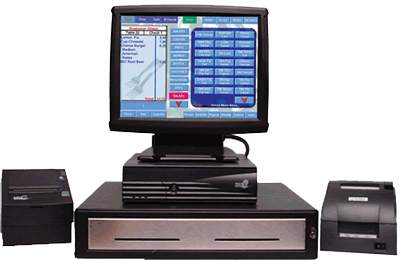
\includegraphics[width=\textwidth]{./img/aloha_pos.png}
	\caption{Przykładowy model kasy Aloha.}
	\label{fig:aloha_pos}
\end{figure}
Terminale kasowe Aloha (rys. \ref{fig:aloha_pos}) są niezwykle popularne w Stanach Zjednoczonych. Umożliwiają one kompleksową obsługę transakcji w sklepie, wpłat oraz wypłat do kasy. Jedną z dodatkowych możliwości terminala jest również dostarczanie informacji o zalogowaniu się pracownika i jego wylogowaniu, co pozwala ustalić intensywność pracy danej osoby, bądź też faktyczne godziny w~jakich pracuje. W systemie 360iQ kasy Aloha wykorzystywane są do sklepach sieci Burger King. Terminal kasy przy każdym tzw. zdarzeniu, wysyła informację do nasłuchującego go kontrolera. Zdarzenia te są prostymi akcjami wykonywanymi podczas użytkowania kasy np. dodanie nowego produktu, potwierdzenie przyjęcia płatności. Dzięki gromadzeniu tych akcji po stronie kontrolera istnieje możliwość połączenia ich w zbiory, które będą reprezentować transakcje, wpłaty, wypłaty oraz obecności pracowników. Łączeniem tych zdarzeń w całość zajmuje się moduł aplikacji zainstalowany na kontrolerze zwany PreParserem, który jako część systemu 360iQ funkcjonuję pod nazwą AlohaPreParser. Przetwarza on zdarzenia uwzględniając zawarte w nich informacje dotyczące numeru kasy, rachunku etc.
Po wstępnym przetworzeniu danych zostają one wysłane do bazy ulokowanej po stronie administratora, gdzie przechwytywane są one przez Parser i dokonywana jest właściwa analiza danych i ich przetwarzanie w celu dostarczenia klientowi potrzebnych informacji. 
\newpage
\subsection{Umiejscowienie w systemie 360iQ}
AlohaPreParser oraz AlohaParser są bezpośrednimi składowymi systemu 360iQ dostarczanemu przez firmę EZUniverse. System ten składa się z~całej infrastruktury nakierowanej na dostarczenie klientowi maksymalnej liczby informacji mogących wesprzeć funkcjonowanie biznesu klienta. Wspierane są duże ilości modeli kas, które mogą być zainstalowane w klepie klienta. Dzięki wsparciu dla dużej ilości modeli kas oraz współpracy z największymi sieciami sklepów (np. Subway, Burger King) system 360iQ jest kompleksowa platformą do wspomagania biznesu klienta.
\subsection{Dane wejściowe}
Danymi wejściowymi dostarczanymi do kontrolera są pojedyncze zdarzenia zapisane w formacie XML (ang. Extensible Markup Language, w wolnym tłumaczeniu Rozszerzalny Język Znaczników)).
Format przychodzących danych omówiony zostanie na podstawie następującego zdarzenia (Rys. \ref{lst:przykladoweZdarzenieAloha}).  
\begin{figure}[t]
	\begin{lstlisting}[frame=single, breaklines=true, numbers=none]
	<SpyMessage 
		TerminalID="3"
		EventTime="18:00:38" 
		EmployeeID="139" 
		EmployeeName="JAMES BOND" 
		ManagerID="0" ManagerName="" 
		TableID="3132860" 
		CheckID="3145860" 
		TransactionTypeID="8" 
		TransactionType="ADD_ITEM" 
		Description="SM FRY" 
		Amount="1.99" 
		Quantity="1" 
		Sender="192.168.0.101" 
		ReceivedOn="2017/03/05 00:00:52.042" 
	/>
	\end{lstlisting}
	\caption{Przykładowe zdarzenie - dane wygenerowane przez kasę Aloha.}
	\label{lst:przykladoweZdarzenieAloha}
\end{figure}
Opisuje ono akcję dodania nowego przedmiotu do rachunku o numerze 3145860. Możemy na podstawie przedstawionego listingu ustalić również, że dane zdarzenie miało miejsce o godzinie 18:00:38 oraz przedmiot SM FRY został dodany do rachunku przez pracownika JAMES BOND. Na podstawie tak przedstawionych danych wejściowych moduł przetwarzania wstępnego jest w stanie budować całe zestawy transakcji, które zawierają szereg zdarzeń podobnych temu wyżej przedstawionemu. Dzięki tak pogrupowanym danym, zamiana zwykłych zdarzeń z terminala na struktury mogące być poddane analizie jest znacznie uproszczona. Terminal generuje również dodatkowe dane przechwytywane przez kontroler zwane słownikami. Słowniki są zestawami danych zapisanych w formacie XML niosącymi informacje o specyficznych cechach danego sklepu, np. promocjach, identyfikatorach produktów, bądź podatkach. Przykładowe słowniki przedstawiono na listingach w skróconej formie, gdyż całe pliki potrafią zawierać znaczne ilości informacji (: Rys. \ref{lst:przykladowySlownikProduktow} - kategorie produktów, Rys. \ref{lst:przykladowySlownikPromocji} - lista promocji: )
\begin{figure}[t]
	\begin{lstlisting}[frame=single, breaklines=true]
	<ItemCategoryMessage>
		<Item ItemId="484" ItemName="WRP BLT CSP" Price="3.49">
			<Category CategoryId="55" CategoryName="ALL ITEMS" />
			<Category CategoryId="57" CategoryName="DISCOUNTABLE ITEMS" />
			<Category CategoryId="56" CategoryName="ALL ITEMS EXCEPT CMB" />
			<Category CategoryId="25" CategoryName="ALL SALADS" />
			<Category CategoryId="1" CategoryName="FOOD" />
		</Item>
		<Item ItemId="5748" ItemName="AVOCADO RAN" Price="0">
			<Category CategoryId="55" CategoryName="ALL ITEMS" />
			<Category CategoryId="57" CategoryName="DISCOUNTABLE ITEMS" />
			<Category CategoryId="56" CategoryName="ALL ITEMS EXCEPT CMB" />
			<Category CategoryId="1" CategoryName="FOOD" />
		</Item>
	</ItemCategoryMessage>
	\end{lstlisting}
	\caption{Przykładowy słownik produktów w formacie XML - wersja skrócona.}
	\label{lst:przykladowySlownikProduktow}
\end{figure}

\begin{figure}[t]
	\begin{lstlisting}[frame=single, breaklines=true]
	<PromotionMessage>
		<Item ItemId="7592" ItemName="Items" Price="0">
			<Promotion PromotionId="6485" PromotionVersion="1941" PromotionName="6485*$5C'wich Ml 2" />
			<Promotion PromotionId="118" PromotionVersion="999" PromotionName="Local Combos" />
			<Promotion PromotionId="139" PromotionVersion="2655" PromotionName="Bacon King" />
			<Promotion PromotionId="101" PromotionVersion="689" PromotionName="Whopper Combo" />
			<Promotion PromotionId="108" PromotionVersion="693" PromotionName="Orig. Chicken Combo" />
			<Promotion PromotionId="221" PromotionVersion="93" PromotionName="Crois'wich Combo" />
		</Item>
	</PromotionMessage>
	\end{lstlisting}
	\caption{Przykładowy słownik listy promocji w formacie XML - wersja skrócona.}
	\label{lst:przykladowySlownikPromocji}
\end{figure}
Słowniki te gromadzone są przez moduł wstępnego przetwarzania i wykorzystywane w analizie wspomnianych wcześniej danych wejściowych i algorytmach mających na celu dokonanie odpowiednich poprawek w danych transakcyjnych (szczegółowo ten temat został poruszony w rozdziale \ref{rozdzial5} traktującym o wykorzystanych algorytmach).
\subsection{Typy zdarzeń generowanych przez kasę Aloha}
Kasa Aloha jest zdolna do wygenerowania szeregu typów zdarzeń. Są to między innymi:
\begin{itemize}
	\setlength\itemsep{0.1pt}
	\item Zalogowanie pracownika w kasie.
	\item Wylogowanie pracownika z kasy.
	\item Przerwa w pracy.
	\item Zakończenie przerwy w pracy.
	\item Otwarcie kasy.
	\item Dodanie nowego przedmiotu do transakcji.
	\item Anulowanie dodanego przedmiotu.
	\item Usunięcie przedmiotu z transakcji.
	\item Otwarcie nowego zamówienia.
	\item Drukowanie rachunku.
	\item Zamknięcie zamówienia.
	\item Ponowne otwarcie zamówienia.
	\item Przyjęcie płatności.
	\item Autoryzacja płatności.
	\item Odrzucenie płatności.
	\item Modyfikacja płatności.
	\item Usunięcie płatności.
	\item Dodaj promocje.
	\item Usuń promocje.
	\item Wartość podatku.
	\item Wartość netto transakcji.
	\item Wartość brutto transakcji.
	\item Dodatek do potrawy.
\end{itemize}
Jest to lista wszystkich obsługiwanych typów zdarzeń. Są one identyfikowane przez PreParser na podstawie przypisanych im unikalnych identyfikatorów. Istnieje  jeden typ zdarzenia, który nie został uwzględniony w wyżej wymienionej liście, mianowicie zdarzanie nie będące elementem transakcji zakończonej sprzedażą. Takie przypadki to tzw. transakcje typu NO\_SALE i są  one analizowane z~wykorzystaniem szczególnego podejścia. Jest ono szerzej opisane w rozdziale \ref{rozdzial5}.
\subsection{Etap wstępnego przetwarzania}
Każdy sklep korzystający z oprogramowania będącego przedmiotem niniejszej pracy wymaga instalacji specjalnego modułu działającego jako serwis na komputerze zwanym kontrolerem. Urządzenie to gromadzi zdarzenia generowane przez kasy działające w obrębie omawianego sklepu. Odebrane informacje są przechwytywane przez działający w systemie moduł wstępnego przetwarzania, który poddaje je wstępnej analizie. Możemy wyodrębnić kluczowe etapy składające się na przeprowadzenie wspomnianego procesu:
\begin{itemize}
	\item Sprawdzanie danych pod kątem duplikatów i ich odpowiednie odfiltrowanie.
	\item Analiza możliwości wystąpienia niezamkniętych lub błędnych transakcji i~ich odpowiednia obsługa.
	\item Grupowanie zdarzeń przychodzących z kasy w kolekcje związane z jedną transakcją.
	\item Przeszukiwanie transakcji, które zostały pogrupowane i sprawdzanie czy wymagana jest korekcja cen produktów lub płatności.
	\item Przetwarzanie całych grup transakcji, rozbudowa zdarzeń z wykorzystaniem algorytmów analizy promocji oraz kategorii produktów.
	\item Konwersja zgrupowanych zdarzeń na obiekty XML (transakcje, wpłaty~/wypłaty z kasy, obecności pracowników).
	\item Wysyłanie XMLi do bazy danych w celu ich przetworzenia przez moduł właściwego przetwarzania.
\end{itemize}
\subsection{Etap właściwego przetwarzania}
Po wstępnym przetworzeniu danych, gdy moduł wstępnego analizowania informacji przekaże je do bazy danych udostępnianej przez administratora systemu, są one przechwytywane przez działający w środowisku dostarczyciela usługi moduł właściwego przetwarzania danych. Pobiera on z tabel dane w~formacie XML, które dzięki wstępnej pracy wykonanej przez PreParser są już odpowiednio pogrupowane i oznaczone. Umożliwia to Parserowi wejście na poziom wyżej w analizie danych, podczas gdy PreParser analizował zdarzenia pod kątem grupowania ich w struktury, Parser może analizować same zdarzenia i wyciągać z~nich informacje, które są konieczne do zbudowania wyczerpującego opisu transakcji, bądź innego zdarzenia, które miało miejsce na kasie.
Moduł ten analizuje każde zdarzenie i krok po kroku tworzy obiekt, który na sam koniec przetwarzania danych zostanie umieszczony w wynikowej bazie. Udostępnia ona bezpośrednio dane mogące być analizowane przez klienta za pośrednictwem specjalnej aplikacji webowej będącej częścią systemu 360iQ. Schemat analizy danych przez moduł właściwego przetwarzania wygląda następująco:
\begin{itemize}
\item Sprawdzanie danych pod kątem duplikatów i ich odpowiednie odfiltrowanie.
\item Wykrywanie typu zdarzenia jakie zostało zgrupowane w wejściowy XML: (transakcja, wpłata/wypłata, obecność pracownika).
\item Uruchamianie odpowiedniego schematu przetwarzania zależnie od wykrytego typu wiadomości.
\item Analiza danych w formacie XML krok po kroku i tworzenie cyfrowego modelu będącego odpowiednikiem realnej czynności wykonanej przez pracownika sklepu.
\item Sprawdzanie poprawności stworzonych modeli i dokonywanie koniecznych poprawek, jak również oznaczenie tych, które zawierają wartości odbiegające od normy (ten fakt jest później odpowiednio prezentowany użytkownikowi w aplikacji webowej).
\item Generowanie paragonów do wglądu przez klienta.
\item Wysyłanie przetworzonych modeli do odpowiednich tabel wynikowej bazy danych w zależności od typu przetwarzanych wiadomości.
\end{itemize}
\subsection{Przypadki niestandardowe}
Terminale kasowe Aloha są dość bogate w przypadki, które można uznać za niestandardowe. Do najczęstszych takich sytuacji możemy zaliczyć:
 \begin{itemize}
 	\item Wadliwe dane wejściowe,
 	\item Niezamknięte transakcje,
 	\item Dodawanie przedmiotów do rachunku z użyciem ich pełnej nazwy oraz późniejsze usuwanie z wykorzystaniem jej skróconej wersji,
 	\item Dodawanie promocji bez uwzględnienia odpowiednich przedmiotów, które powinna dodana promocja dodawać,
 	\item W regionach innych niż Stany Zjednoczone częstym problemem jest brak informacji o podatkach.
 \end{itemize}
\subsubsection{Wadliwe dane wejściowe}
Z racji faktu, że moduł wstępnego przetwarzania otrzymuje dane z terminali kasowych Aloha w formacie XML, często zdarza się sytuacja, że jest on wadliwy (np. ucięty) lub też występują jego duplikaty. W takich przypadkach PreParser ustawia odpowiednie statusy tych wiadomości (mogą być one potem zweryfikowane przez użytkownika) i pomija je w procedurze wstępnej analizy.
\subsubsection{Niezamknięte transakcje}
Jednym z najrzadziej występujących przypadków niestandardowych jest sytuacja, gdy mamy do czynienia z niezamkniętą transakcją. Dzieje się to wtedy, gdy otwierana jest transakcja, lecz nie przychodzi zdarzenie oznaczające jej zamknięcie (w Aloha jest to: CLOSE\_CHECK). W takiej sytuacji moduł wstępnego przetwarzania ustawia taką transakcję w stan oczekiwania, który trwa 24 godziny. Jeśli do tego czasu przyjdzie zdarzenie zamykające daną transakcję, to zostanie ona zatwierdzona i przesłana do dalszej analizy, w przeciwnym razie nastąpi jej usunięcie z kolejki oczekujących i oznaczenie jako błędnej danej wejściowej, by użytkownik mógł samodzielnie się jej przyjrzeć.
\subsubsection{Dodawanie przedmiotów do rachunku z użyciem ich pełnej nazwy oraz późniejsze usuwanie, przy wykorzystaniu ich skróconej nazwy}
Przedmioty dodawane przez kasę Aloha do rachunków niestety często charakteryzują się niejednolitym nazewnictwem. Ten sam przedmiot może być nazywany z wykorzystaniem:
 \begin{itemize}
	\item nazwy skróconej,
	\item pełnej nazwy przedmiotu,
	\item ID przedmiotu, bądź jego oznaczenia kodowego.
\end{itemize}
Powoduje to problemy przy usuwaniu z rachunku już dodanych przedmiotów. Przedmiot dodany do transakcji pod nazwą X może być z niej usuwany pod nazwą Y. W celu uzyskania spójności i powiązania ze sobą przedmiotów wykorzystywany jest algorytm rozszerzania danych przekazywanych przez zdarzenie. Korzysta on ze słownika kategorii przedmiotów, który jest dostarczany raz dziennie przez właściciela sklepu jako specjalne zdarzenie terminala Aloha i przechowywany przez kontroler. Dzięki temu słownikowi możliwe jest powiązanie ze sobą tych samych przedmiotów występujących pod różną nazwą, wykorzystując fakt, że każdy przedmiot ma swoje unikalne ID, które jest udostępniane za pośrednictwem słownika kategorii produktów. Takie rozwiązanie gwarantuje, że w wynikowej transakcji przedmioty będą powiązane i usunięte w sposób prawidłowy niezależnie od zastosowania pełnej, bądź jego skróconej nazwy.
\subsubsection{Dodawanie promocji bez uwzględnienia odpowiednich przedmiotów, które określona promocja powinna dodawać}
Niezbyt przyjazną cechą terminala Aloha jest obsługa dodawania promocji bez uwzględnienia przedmiotów wchodzących w jej skład. W takim wypadku konieczne jest dodanie przedmiotów do transakcji, których dotyczy dana promocja, dzięki czemu zachowana zostanie zgodność danych z realnie sprzedanymi przedmiotami po stronie sklepu. Dodawanie przedmiotów przez moduł wstępnego przetwarzania realizowane jest przy użyciu słownika promocji dostarczanego przez klienta dla każdego sklepu. Pozwala on zidentyfikować nazwę promocji i rozszerzyć XML z transakcją o potrzebne przedmioty. 
\subsubsection{W regionach innych niż Stany Zjednoczone częstym problemem jest brak informacji o podatkach}
Problem ten objawia się sytuacją, gdy w zdarzeniu wystawianym przez terminal mającym typ "TAX" pojawia się zerowa wartość podatku. W tej sytuacji, by uzyskać prawidłową cenę końcową z wliczoną już wartością podatku, konieczne jest wczytanie dodatkowego słownika przechowującego wartości podatków dla każdego z przedmiotów. Takie rozwiązanie pojawia się w sytuacji, gdy oprogramowanie działa w krajach gdzie system podatkowy znacząco różni się od tego, który obowiązuje w Stanach Zjednoczonych. 
\section{Opis technologii i wykorzystanych narzędzi}
\subsection{Środowisko pracy i język programowania}
Projekt został zrealizowany przy użyciu technologii .NET (\cite{aspnet}, \cite{aspnet}) oraz języka C\# (\cite{ruszglowa}).
Wielokrotnie podczas przeglądania kodu źródłowego projektu można również napotkać skrypty pisane w języku T-SQL (\cite{tsql}), w celu komunikacji z bazą danych.
Całość projektu została napisana w środowisku Visual Studio 2017, przy czym korzystano również z Visual Studio Code w celu analizy danych XML oraz szybkiego przeglądania plików tekstowych.
Do administrowania i zarządzania bazą danych wykorzystano Microsoft SQL Server Management Studio 2016.
Podczas projektowania algorytmów i optymalizacji kodu wykorzystywano wiedzę zdobytą w wyniku lektury lektur: (\cite{algorytmy}, \cite{perelki}, \cite{wzorceprojektowe}).
Dodatkowo w celu poprawnej implementacji serwisu działającego w środowisku Windows korzystano z pozycji - (\cite{progwin})
Wybór narzędzi wynikał ze standardów panujących firmie EZUniverse, na zlecenie której tworzone jest oprogramowanie.
\subsection{Baza danych}
Serwerem bazy danych był Microsoft SQL Server 2016 w wersji Express zainstalowany na lokalnym komputerze. Dokonano połączenia, na lokalnej bazie developera, tabel koniecznych do pracy modułu wstępnego przetwarzania i tych niezbędnych do funkcjonowania jednostki realizującej właściwe procesowanie danych.
Dzięki takiemu rozwiązaniu można było testować działanie całego systemu na lokalnym komputerze bez konieczności korzystania z osobnego komputera, który miałby pełnić funkcję kontrolera.
Dane wykorzystywane w niniejszym projekcie są kopią zapasową rzeczywistych danych źródłowych zaczerpniętych z codziennej pracy systemu u klienta. Pozwala to testować i przedstawić pracę niniejszego projektu w jego naturalnych warunkach i w starciu z prawdziwymi danymi generowanymi przez sklepy w Stanach Zjednoczonych.
\subsection{Moduły wspierające}
Opisywana w niniejszej pracy aplikacja jest wspierana przez następujące oprogramowanie, które jest częścią systemy 360iQ i zostało opracowane przez firmę EZUniverse:
 \begin{itemize}
 	\item AlohaSpyRelay,
 	\item EZ360DataInterface.
 \end{itemize}
\subsubsection{AlohaSpyRelay}
AlohaSpyRelay jest aplikacją zapewniającą transmisje danych z kasy Aloha do kontrolera gdzie zainstalowany jest moduł wstępnego przetwarzania. Pobiera ona dane bezpośrednio z terminala, zamienia ja na zdarzenia zapisane w formacie XML i przekazuje do kontrolera.
\subsubsection{EZ360DataInterface}
EZ360DataInterface jest łącznikiem pomiędzy modułem wstępnego przetwarzania i częścią odpowiadająca za właściwe przetwarzanie. Po wstępnym przetworzeniu danych przez PreParser istnieje konieczność wysłania ich do bazy danych dostarczanej przez administratora systemu, tym właśnie zajmuje się opisywana aplikacja. Moduł wstępnego przetwarzania przygotowuje gotową paczkę danych do wysłania i powiadamia EZ360DataInterface, że są dane do wysyłki. Aplikacja przechwytuje dane od PreParsera i wysyła je zgodnie ze skonfigurowanymi w jej ustawieniach wytycznymi.
\chapter{Wymagania}
\label{rozdzial3}
Rozdział ten opisuje wymagania konieczne do uruchomienia oprogramowania po stronie kontrolera jak i administratora aplikacji. Przedstawione zostały również przypadki użycia oprogramowania przez użytkownika wraz ze stosownym komentarzem.
\section{Wymagania funkcjonalne}
\subsection{Moduł wstępnego przetwarzania danych - PreParser}
Wymagania funkcjonalne odnośnie modułu PreParsera składają się z następujących założeń:
\begin{itemize}
	\item Serwis powinien być wstanie odczytywać pobrane dane z lokalnej bazy danych kontrolera, gdzie przechowywane są informację o zdarzeniach, które nadesłał terminal Aloha,
	\item Powinna istnieć możliwość przetwarzania dany na etapie wstępnej analizy w celu eliminacji duplikatów i wadliwych wiadomości.
	\item Kluczową kwestią jest zastosowanie algorytmów dodających brakujące produkty z promocji oraz rozszerzające nazwy wspomnianych wcześniej produktów, by można było je łatwo ze sobą powiązać.
	\item Serwis powinien informować użytkownika na bieżąco o stanie swojej aktywności za pośrednictwem komunikatów w pliku logów.
	\item Serwis powinien być zdolny grupować wiadomości w kolekcje i konwertować je na odpowiednio zdefiniowane XMLe, a następnie wysyłać je do bazy danych po stronie administratora, by mogły być one dalej analizowane.
\end{itemize}
\subsection{Moduł właściwego przetwarzania danych - Parser}
Podczas projektowania modułu Parsera powinny zostać uwzględnione następujące wymagania funkcjonalne:
\begin{itemize}
	\item Aplikacja powinna móc odczytywać dane z odpowiednich tabel w bazie danych, gdzie w sposób ciągły pojawiają się nowe dane przysyłane z bliżej nie określonej liczby kontrolerów, gdzie zostały one wstępnie obrobione przez moduł wstępnego przetwarzania.
	\item Oprogramowanie musi wspierać różne typy przychodzących wiadomości (transakcje, wpłaty/wypłaty, obecności pracowników) i stosować dla nich właściwe formy analizy i przetwarzania.
	\item Wynikowe dane powinny zostać zapisane w bazie danych, z której może korzystać aplikacja webowa dostarczana jako element systemu 360iQ i~opracowana przez firmę EZUniverse i prezentująca wyniki użytkownikowi w~przyjaznej dla niego formie. Rezultat przetwarzania powinien być możliwie jak najdokładniejszym odwzorowaniem zdarzenia jakie zaszło w danej chwili czasu na kasie w sklepie użytkownika. Ważne jest zachowanie odpowiednich stref czasowych i synchronizacja czasu wideo,
	\item W przypadku wystąpienia błędu podczas analizy danych, aplikacja powinna zamieści odpowiednią informację na ekranie interfejsu użytkownika.
\end{itemize}
\section{Wymagania niefunkcjonalne}
\subsection{Moduł wstępnego przetwarzania danych - PreParser}
Wymagania niefunkcjonalne odnośnie modułu PreParsera składają się z następujących założeń:
\begin{itemize}
	\item Stabilnie działający serwis po stronie kontrolera.
	\item Personalizacja za pomocą jednego pliku konfiguracyjnego.
	\item Prosty sposób instalacji oraz włączania serwisu.
	\item Szczegółowy system logów pomagający w diagnostyce usterek i monitoringu działania aplikacji.
	\item Niskie wymagania sprzętowe, serwis powinien się uruchamiać i pracować bez widocznych strat na wydajności będąc zainstalowanym na stosunkowo taniej i mało wydajnej maszynie.
\end{itemize}
\subsection{Moduł właściwego przetwarzania danych - Parser} 
Podczas projektowania modułu Parsera powinny zostać uwzględnione następujące wymagania niefunkcjonalne:
 \begin{itemize}
 	\item Stabilnie działająca aplikacja desktopowa z intuicyjnym interfejsem użytkownika.
 	\item Pełne wsparcie dla przetwarzania danych z kas Aloha oraz integracja z~pozostałymi parserami z innych kas działającymi w systemie.
 	\item Prosty i intuicyjny interfejs użytkownika.
 	\item Łatwość wystartowania i zatrzymania aplikacji.
 	\item Dążenie do jak najniższego wykorzystania zasobów systemu, w którym aplikacja jest zainstalowana.
 \end{itemize}
\section{Analiza przypadków użycia (diagramy UML)}
W niniejszej sekcji zaprezentowano przypadki użycia dla modułu wstępnego przetwarzania(rys. \ref{fig:przypadki_uzycia_preparser}). Schemat dla modułu PreParsera obrazuje czynności możliwe do wykonania przez użytkownika aplikacji w celu sterowania jej pracą. Natomiast diagram dla części odpowiadającej za właściwe przetwarzanie (rys. \ref{fig:przypadki_uzycia_parser}) pokazuje akcje i czynności, jakie może podjąć administrator, by kontrolować pracę Parsera.
\begin{figure}[t]
	\centering
	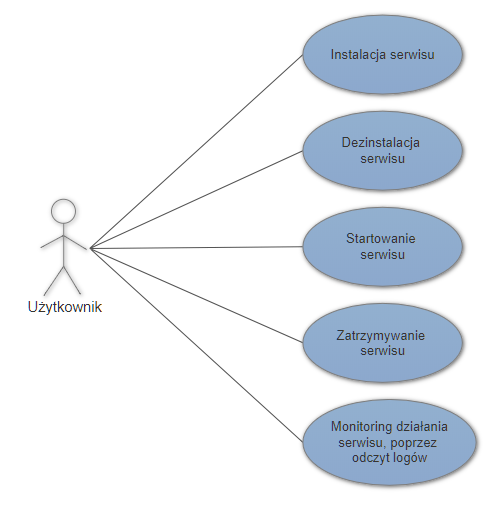
\includegraphics{./img/przypadki_uzycia_preparser.png}
	\caption{Przypadki użycia - moduł wstępnego przetwarzania.}
	\label{fig:przypadki_uzycia_preparser}
\end{figure}
\begin{figure}[t]
	\centering
	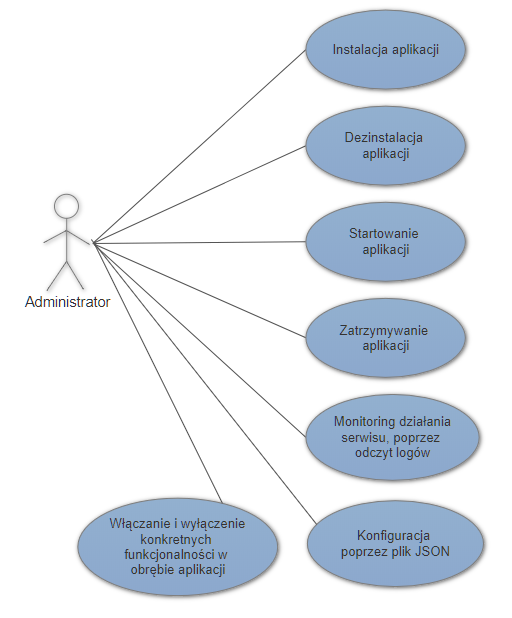
\includegraphics{./img/przypadki_uzycia_parser.png}
	\caption{Przypadki użycia - moduł właściwego przetwarzania.}
	\label{fig:przypadki_uzycia_parser}
\end{figure}
\chapter{Specyfikacja zewnętrzna}
\label{rozdzial4}
Rozdział ten opisuje wymagania sprzętowe i programowe, które należy spełnić, by zapewnić poprawne funkcjonowanie aplikacji. Poruszone zostały kwestie instalacji i administracji poszczególnymi modułami oprogramowania oraz temat zabezpieczeń.
\section{Wymagania sprzętowe i programowe}
Opisywana aplikacja została przetestowana, na dwóch konfiguracjach sprzętowych:
 \begin{itemize}
	\item Komputer stacjonarny:
	\subitem Procesor - i5 4690K @ 4.5 GHz, 4.4GHz Uncore,
	\subitem Pamięć RAM - 8GB DDR3 @ 2133MHz CL9.11.12 T1,
	\subitem Dysk - SSD 128 GB TLC,
	\subitem System operacyjny - Windows 10 PRO.
	\item Laptop:
	\subitem Procesor - i5 7200U @ 2.5 GHz,
	\subitem Pamięć RAM - 16GB DDR4 @ 2133MHz CL15,
	\subitem Dysk - SSD 256 GB MLC,
	\subitem System operacyjny - Windows 10 PRO.
\end{itemize}
Obydwie konfiguracje gwarantowały satysfakcjonującą płynność i szybkość działania aplikacji.
Na podstawie testów z użyciem wyżej wymienionych zestawów zdefiniowano przybliżone wymagania sprzętowe oraz programowe:
\begin{itemize}
	\item Minimalne wymagania sprzętowe:
	\subitem Procesor - i3 2 generacji Intel Core lub odpowiednik AMD,
	\subitem Pamięć RAM - 4GB pamięci operacyjnej,
	\subitem Dysk - 100MB wolnej przestrzeni dyskowej,
	\subitem Stały dostęp do internetu.
	\item Minimalne wymagania programowe:
	\subitem System operacyjny - Windows w wersji 7 lub nowszej,
	\subitem Microsoft SQL Server Management Studio oraz MS SQL Server w~wersji 2012 lub nowszej,
	\subitem .NET Framework w wersji 3.5 lub nowszej.
\end{itemize}
\section{Instalacja}
\subsection{Instalacja PreParser-a na kontrolerze u klienta}
W celu zainstalowania  modułu wstępnego przetwarzania danych należy uruchomić plik EZ360PreParserService.Setup.v.VERSION.exe, gdzie VERSION jest numerem wersji.
Uruchomionony zostanie instalator serwisu (rys. \ref{fig:preparser_installation_part1}). W momencie wciśnięcia przycisku Install, instalator rozpocznie wgrywanie PreParser na kontroler. Po zakończeniu procesu powinien zostać wyświetlony ekran informujący o poprawnie zakończonej instalacji serwisu (rys. \ref{fig:preparser_installation_part2})
\begin{figure}[t]
	\centering
	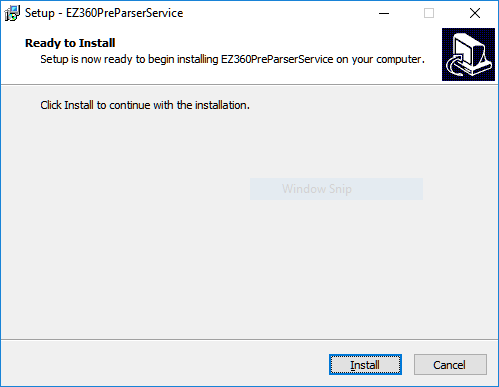
\includegraphics[width=\textwidth]{./img/preparser_installation_part1.png}
	\caption{Instalacja modułu wstępnego przetwarzania - początek instalacji.}
	\label{fig:preparser_installation_part1}
\end{figure}
\begin{figure}[t]
	\centering
	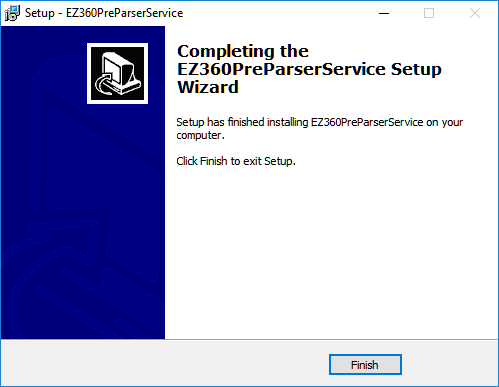
\includegraphics[width=\textwidth]{./img/preparser_installation_part2.png}
	\caption{Instalacja modułu wstępnego przetwarzania - koniec instalacji.}
	\label{fig:preparser_installation_part2}
\end{figure}
Następnie należy dokonać konfiguracji zainstalowanego serwisu. W tym celu otwieramy plik configuration.json. Powinien on mieć format przedstawiony na rys. \ref{lst:przykladowyPlikKonfiguracyjnyPreParser}.
\begin{figure}[t]
	\begin{lstlisting}[frame=single, breaklines=true]
	{
	"ProcessID": 636298774975,
	"ParserType": "ALOHA",
	"ObjectsConnectionString": "Data Source = source; User ID = sa; Password = sa; Initial Catalog = EZ360Objects;",
	"CommunicationConnectionString": "Data Source = source; User ID = sa; Password = sa; Initial Catalog = EZ360Communication;",
	"TransactionWebservice": "http://localhost:65059/api/Transactions",
	"ActionWebservice": "http://localhost:65059/api/Actions",
	"CashOperationWebservice": "http://localhost:65059/api/CashOperations",
	"TimeClockWebservice": "http://localhost:65059/api/TimeClocks",
	"DataWebservice": "http://localhost:65059/api/Data",
	"TimerInterval": 500,
	"DatabaseTimeout": 30,
	"DatabaseTimeoutInterval": 10,
	"DelayAfterDatabaseError": 10,
	"DelayDeleteNotServedTransaction": 40,
	"Rows": 500,
	"SenderTimerInterval": 1000,
	"MaxRowsToSend": 25,
	"MaxSenderQueues": 250,
	"CompressWebRequest": true,
	"ControllerWebURL": "http://127.0.0.1:81/"
	}
	\end{lstlisting}
	\caption{Zawartość pliku konfiguracyjnego - PreParser.}
	\label{lst:przykladowyPlikKonfiguracyjnyPreParser}
\end{figure}
Skrócony opis poszczególnych parametrów:
\begin{itemize}
	\setlength\itemsep{0.1pt}
	\item ProcessID - id procesu działającego na danym kontrolerze.
	\item ParserType - typ parsera komunikującego się z kontrolerem.
	\item ObjectsConnectionString - parametry połączenia do tabeli EZ360Objects w bazie danych.
	\item CommunicationConnectionString - parametry połączenia do tabeli \newline EZ360Communication w bazie danych.
	\item TransactionWebservice - adres url do webservice-u obsługującego transakcje.
	\item ActionWebservice - adres url do webservice-u obsługującego akcje.
	\item CashOperationWebservice - adres url do webservice-u obsługującego wpłaty/wypłaty.
	\item TimeClockWebservice - adres url do webservice-u obsługującego obecności pracowników.
	\item DataWebservice - adres url do webservice-u obsługującego dane dodatkowe.
	\item TimerInterval - czas pomiędzy kolejnymi sprawdzeniami czy nie przyszły nowe zdarzenia (w milisekundach).
	\item DatabaseTimeout - maksymalny czas w jakim może zostać wykonywane zapytanie do bazy danych (w sekundach).
	\item DatabaseTimeoutInterval - przerwa pomiędzy kolejnymi zapytaniami do bazy danych (w sekundach).
	\item DelayAfterDatabaseError - czas do ponownej próby połączenia z bazą danych po wystąpieniu błędu.
	\item DelayDeleteNotServedTransaction - czas po jakim nieobsługiwana transakcja jest usuwana.
	\item Rows - maksymalna liczba wierszy możliwa do procesowania.
	\item SenderTimerInterval - interwał z jakim wysyłane są dane do bazy.
	\item MaxRowsToSend - maksymalna liczba wierszy przesłana w jednym zapytaniu.
	\item MaxSenderQueues - limit liczby obiektów w kolejce do wysłania.
	\item CompressWebRequest - kompresowanie wysyłanych danych.
	\item ControllerWebURL - adres URL kontrolera.
\end{itemize}
\subsection{Instalacja Parser-a po stronie administratora}
Poprawna instalacja modułu właściwego przetwarzania danych na komputerze administratora wymaga ręcznego rozpakowania archiwum:
\newline
 \texttt{AlohaParser\_VERSION.zip}
 \newline
 Gdzie VERSION jest numerem wersji. Po rozpakowaniu archiwum w miejscu wybranym przez administratora, powinny być dostępne pliki potrzebne do uruchomienia modułu właściwego przetwarzania danych.
Aplikacje można uruchomić otwierając plik EZ360ParserUI.exe.
Następnie należy dokonać konfiguracji zainstalowanej aplikacji. W tym celu otwieramy plik configuration.json. Powinien on mieć format przedstawiony na rys. \ref{lst:przykladowyPlikKonfiguracyjnyParser}.
\begin{figure}[t]
	\begin{lstlisting}[frame=single, breaklines=true]
	"ProcessID": 444,
	"ParserType": "ALOHA",
	"Enabled": false,
	"DBConnections": {
		"AccessConnectionString": "Data Source = source; User ID = sa; Password = sa; Initial Catalog = EZ360Access",
		"CommunicationConnectionString": "Data Source = source; User ID = sa; Password = sa; Initial Catalog = EZ360Communication",
		"LaborConnectionString": "Data Source = source; User ID = sa; Password = sa; Initial Catalog = EZ360Labor",
		"ObjectsConnectionString": "Data Source = source; User ID = sa; Password = sa; Initial Catalog = EZ360Objects",
		"SalesConnectionString": "Data Source = source; User ID = sa; Password = sa; Initial Catalog = EZ360Sales",
		"ReportsConnectionString": "Data Source = source; User ID = sa; Password = sa; Initial Catalog = EZ360Reports",      
		"ApplicationsConnectionString": "Data Source = source; User ID = sa; Password = sa; Initial Catalog = EZ360Applications"
	},
	"TimerInterval": 1000,
	"DatabaseTimeout": 10,
	"DatabaseTimeoutInterval": 10,
	"DelayAfterDatabaseError": 5000,
	"EnablePreserveSavedTransactions": false,
	"DeletePreservedTransactionsAfter": 24,
	"VideoTimeOffset": -10,
	"IdentificationPrefix" : "",
	"IdentificationNumber" : "",
	"Actions": {
	"Enabled": false,
	"Rows": 100
	},
	"CashOperations": { "Enabled": true, "Rows": 100 },
	"Transactions": { "Enabled": true, "Rows": 100 },
	"TimeClocks": { "Enabled": true, "Rows": 100 },
	"Data": { "Enabled": true, "Rows": 100 }
	\end{lstlisting}
	\caption{Zawartość pliku konfiguracyjnego - Parser - wycinek dotyczący kasy Aloha.}
	\label{lst:przykladowyPlikKonfiguracyjnyParser}
\end{figure}
Skrócony opis poszczególnych parametrów:
\begin{itemize}
	\setlength\itemsep{0.1pt}
	\item ProcessID - id procesu działającego na komputerze administratora.
	\item ParserType - typ parsera, którego dotyczy konfiguracja.
	\item AccessConnectionString - parametry połączenia do tabeli EZ360Access w~bazie danych.
	\item CommunicationConnectionString - parametry połączenia do tabeli EZ360Communication w bazie danych.
	\item LaborConnectionString - parametry połączenia do tabeli EZ360Labor w~bazie danych.
	\item ObjectsConnectionString - parametry połączenia do tabeli EZ360Objects w bazie danych.
	\item SalesConnectionString - parametry połączenia do tabeli EZ360Sales w bazie danych.
	\item ReportsConnectionString - parametry połączenia do tabeli EZ360Reports w bazie danych.
	\item ApplicationsConnectionString - parametry połączenia do tabeli EZ360Applications w bazie danych.
	\item TimerInterval - czas pomiędzy kolejnymi sprawdzeniami czy nie przyszły nowe dane (w milisekundach).
	\item DatabaseTimeout - maksymalny czas w jakim może zostać wykonywane zapytanie do bazy danych (w sekundach).
	\item DatabaseTimeoutInterval - przerwa pomiędzy kolejnymi zapytaniami do bazy danych (w sekundach).
	\item DelayAfterDatabaseError - czas do ponownej próby połączenia z bazą danych po wystąpieniu błędu.
	\item EnablePreserveSaveTransactions - definiuje czy włączyć funkcjonalność zachowywania transakcji.
	\item DeletePreserveTransactionsAfter - definiuje po jakim czasie powinny być usuwane zachowane transakcje (podane w godzinach).
	\item Rows - maksymalna liczba wierszy możliwa do procesowania.
	\item VideoTimeOffset - przesunięcie w minutach uwzględniane przy wyliczaniu czasu wideo.
	\item IdentificationPrefix - prefix pomagający zidentyfikować dane.
	\item IdentificationNumer - numer pomagający zidentyfikować dane.
	\item Dalsze ustawienia definiują, które typy danych powinny być przetwarzane.
\end{itemize}
\section{Obsługa systemu i administrowanie nim}
\subsection{PreParser}
\subsubsection{Startowanie serwisu}
Startowanie serwisu realizowane jest z wykorzystaniem systemu operacyjnego Windows. Poprawne wystartowanie modułu wstępnego przetwarzania (po jego odpowiedniej konfiguracji) sprowadza się do uruchomienia serwisu za pośrednictwem menadżera serwisów systemu Windows (proces został zaprezentowany na rys. \ref{fig:startowanie_serwisu})
\begin{figure}[t]
	\centering
	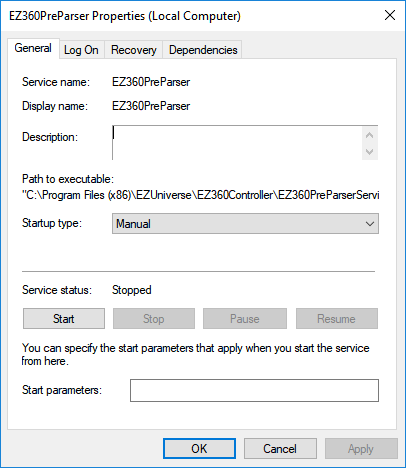
\includegraphics{./img/startowanie_serwisu.png}
	\caption{Przykład startowania/zatrzymywania serwisu.}
	\label{fig:startowanie_serwisu}
\end{figure}
\subsubsection{Zatrzymywanie serwisu}
Zatrzymywanie preparsera realizowane jest podobnie jak jego startowanie. Wykorzystuje się do tego również menadżer serwisów Windows.
\subsubsection{Dezinstalacja serwisu}
W celu usunięcia serwisu z systemu operacyjnego należy uruchomić wiersz poleceń systemu Windows, a następnie przejść do katalogu gdzie został zainstalowany serwis. Po dokonaniu wyżej opisach czynności należy dokonać dezinstalacji poleceniem: \newline
\texttt{EZ360PreParserService.exe -uninstall}
\newline Spowoduje one usunięcie serwisu z systemu. 
\subsubsection{Diagnostyka i logowanie}
Serwis podczas pracy regularnie generuje szereg komunikatów o statusie swojego działania i aktywności.
Są one zapisywane w plikach logów, które przechowywane są w folderze logs. Przechowywanych jest do 30 plików logów, które następnie po pojawieniu się następnych logów są usuwane.
Wyróżniamy następujące typy wiadomości składowanych w logach:
\begin{itemize}
	\item INFO - informuję użytkownika o statusie działa serwisu.
	\item WARN - komunikuje pojawienie się problemu podczas analizy danych, co w większości przypadków oznacza brak wsparcia dla konkretnego typu danych i nie powoduje błędnego działania systemu.
	\item ERROR - zawiadamia o wystąpieniu poważnego problemu, który powinien zostać zgłoszony do administratora w celu jego rozwiązania.
\end{itemize}
\subsection{Parser}
\subsubsection{Uruchamianie aplikacji}
W celu uruchomienia aplikacji należy otworzyć plik EZ360ParserUI.exe, następnie dokonać inicjalizacji poprzez kliknięcie odpowiedniego przycisku.
Po poprawnej inicjalizacji modułu, wystarczy wcisnąć przycisk start, by rozpocząć proces przetwarzania danych (rys. \ref{fig:zatrzymywanie_aplikacji})
\subsubsection{Zatrzymywanie aplikacji}
Administrator może w każdej chwili zatrzymać moduł właściwego przetwarzania danych. W celu dokonania tego, należy kliknąć przycisk STOP (rys. \ref{fig:zatrzymywanie_aplikacji}). Aplikacja dokończy obecny proces przetwarzania i wyśle dane, następnie zatrzyma się (trwa to około kilka sekund, zależnie od ilości przetwarzanych danych).
\begin{figure}[t]
	\centering
	\hspace*{-4.5cm}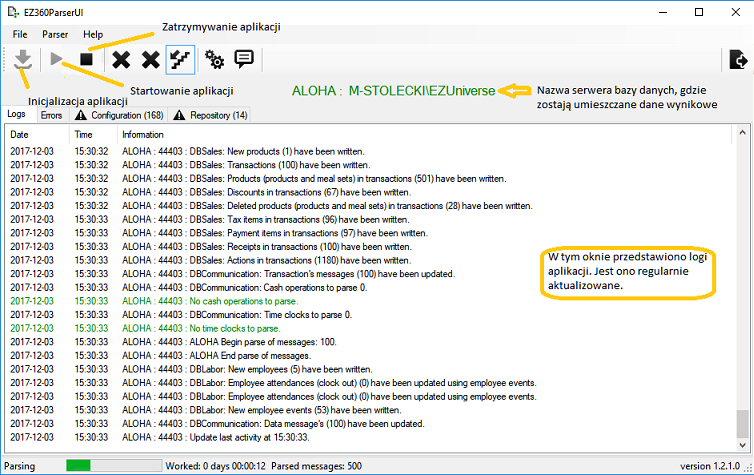
\includegraphics{./img/zatrzymywanie_aplikacji.png}
	\caption{Inicjalizacja/Startowanie/Zatrzymywanie aplikacji}
	\label{fig:zatrzymywanie_aplikacji}
\end{figure}
\subsubsection{Dezinstalacja aplikacji}
Dezinstalacja aplikacji sprowadza się do usunięcia zawartości folderu, w którym został zainstalowany moduł. Należy przy tym pamiętać, by wcześniej zatrzymać Parser i zamknąć aplikację.
\subsubsection{Diagnostyka i logowanie}
Podobnie jak w przypadku modułu wstępnego przetwarzania, tutaj również zaimplementowano system logowania komunikatów. Komunikaty informujące o~stanie działania aplikacji przechowywane są w folderze logs oraz wyświetlane w interfejsie użytkownika, który udostępnia oprogramowanie. W tym wypadku typy komunikatów wyświetlane użytkownikowi są określane przez odpowiedni kolor czcionki:
 \begin{itemize}
 	\item INFO - czarny,
 	\item WARN - zielony,
 	\item ERROR -czerwony.
 \end{itemize}
\section{Bezpieczeństwo}
Ważną kwestią uwzględnianą podczas procesu tworzenia oprogramowania będącego przedmiotem niniejszej pracy jest bezpieczeństwo. W celu zapewnienia uwarunkowań sprzyjających bezpieczeństwu przetwarzanych danych moduł właściwego przetwarzania oraz wszystkie bazy przechowujące informacje przychodzące od strony użytkownika składowane są po stronie administratora systemu. Zapewnia on szereg zabezpieczeń i ciągłe wsparcie techniczne. Po stronie użytkownika zainstalowany jest tylko serwis modułu wstępnego przetwarzania na kontrolerze, który tylko przetwarzana lokalne dane i wysyła je do głównego centrum danych, więc nie ma możliwości dostępu do informacji zgromadzonych przez innych użytkowników.
\section{Przykład działania}
Przykłady działania aplikacji i jej obsługi:
 \begin{itemize}
	\item Startowanie preparsera (rys. \ref{fig:startowanie_serwisu}).
	\item Zatrzymywanie preparsera (rys. \ref{fig:zatrzymywanie_serwisu}).
	\item Startowanie aplikacji (rys. \ref{fig:startowanie_aplikacji}).
	\item Zatrzymywanie aplikacji (rys. \ref{fig:zatrzymywanie_aplikacji}).
	\item Logi modułu wstępnego przetwarzania (rys. \ref{fig:preparser_log}).
	\item Logi modułu właściwego przetwarzania (rys. \ref{fig:parser_log}).
\end{itemize}
\begin{figure}[t]
	\centering
	\hspace*{-5cm}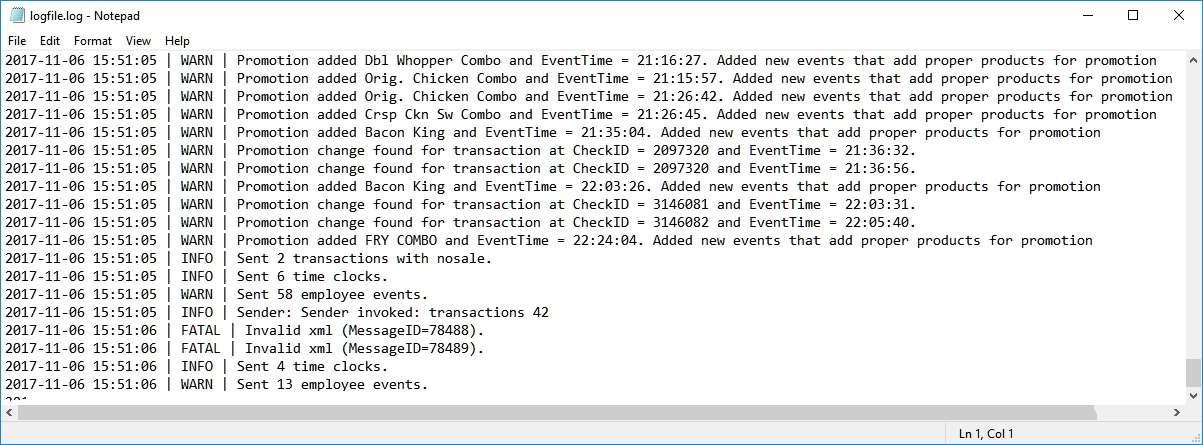
\includegraphics[scale=0.7]{./img/preparser_log.png}
	\caption{Logi PreParsera.}
	\label{fig:preparser_log}
\end{figure}
\begin{figure}[t]
	\centering
	\hspace*{-5cm}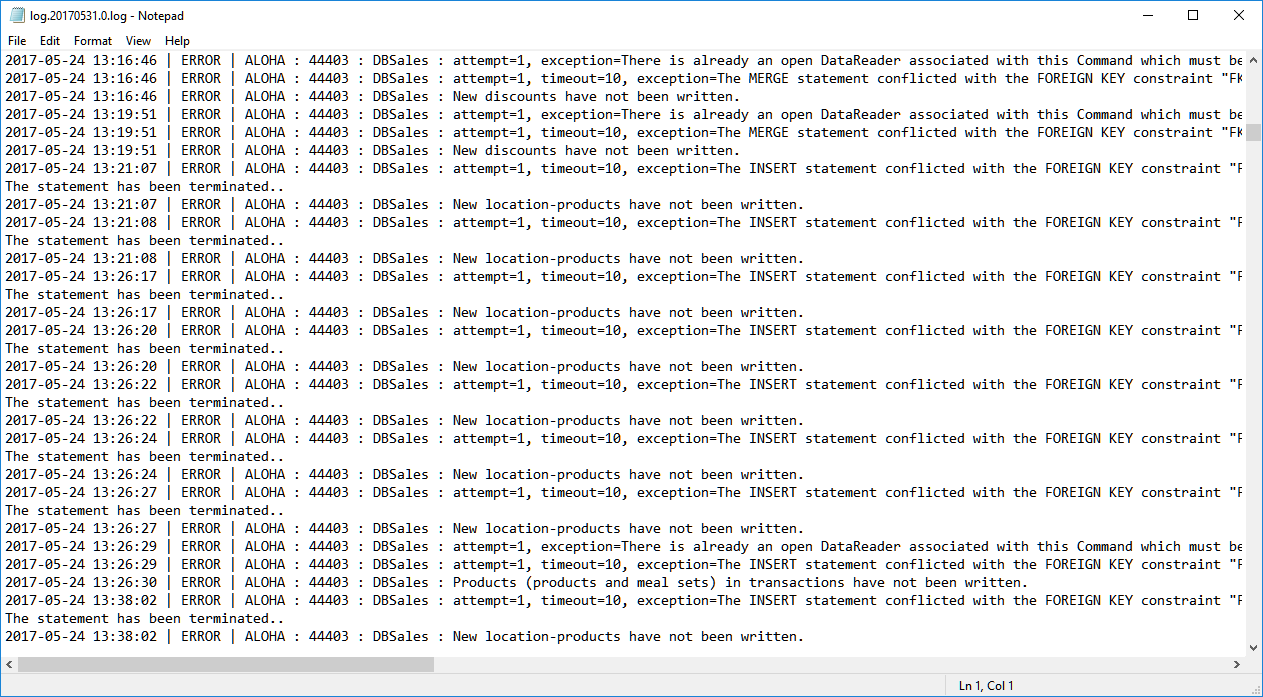
\includegraphics[scale=0.75]{./img/parser_log.png}
	\caption{Logi Parsera.}
	\label{fig:parser_log}
\end{figure}
\chapter{Specyfikacja wewnętrzna}
\label{rozdzial5}
W niniejszym rozdziale podjęta została kwestia architektury oprogramowania. Przedstawione zostały schematy baz danych oraz zakres wykorzystywanych bibliotek. Rozpisano również model ważniejszych klas oraz szczegółowo omówione zostały dane wejściowe wraz z algorytmami koniecznymi do ich odpowiedniej analizy.
\section{Architektura systemu}
Rysunek (rys. \ref{fig:schemat_przeplywu_danych}) przedstawia przepływ danych w systemie realizującym przetwarzanie informacji z kas Aloha.
Jak już wielokrotnie wspominano w niniejszej pracy, dane wychodzące z terminala kasy Aloha mają pewną ścieżkę, którą muszą pokonać zanim zostaną one przekształcone w model, mogący być prezentowany użytkownikowi i analizowany przez niego. Wspominany proces wygląda następująco:
 \begin{enumerate}
	\item Terminal kasy Aloha wysyła komunikat o zdarzeniu.
	\item AlohaSpyRelay przechwytuje informację przychodzącą z terminala i przetwarza ją na format rozpoznawalny przez moduł wstępnego przetwarzania.
	\item Moduł wstępnego przetwarzania zainstalowany na kontrolerze odczytuje dane przychodzące z terminala i opracowane przez AlohaSpyRelay, a następnie dokonuje ich wstępnej analizy.
	\item Dane wynikowe z PreParser przekazywane są do EZ360DataInterface, który przesyła je do bazy danych ulokowanej po stronie administratora systemu.
	\item Moduł właściwego przetwarzania danych odczytuje z bazy wiadomości i~przetwarza je na format mogący być analizowany i oglądany przez użytkownika.
	\item Dane wyjściowe z Parsersa prezentowane są w aplikacji webowej, będącej częścią systemu 360iQ dostarczanego przez firmę EZUniverse.
\end{enumerate}
\begin{figure}[t]
	\centering
	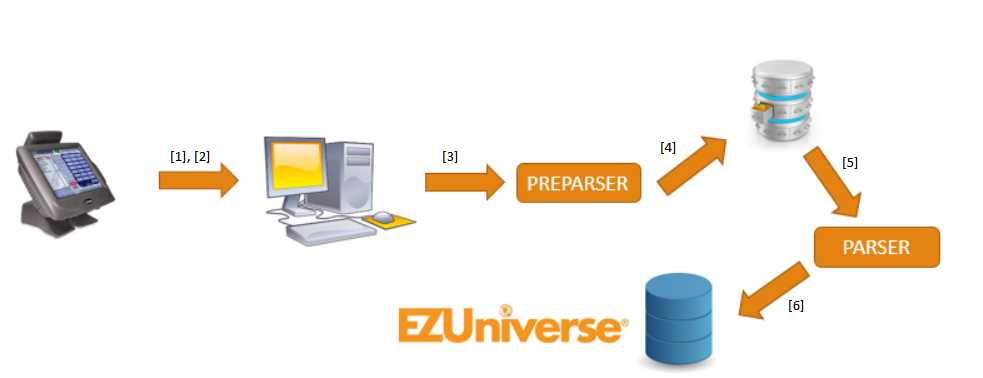
\includegraphics[width=\textwidth]{./img/schemat_przeplywu_danych.png}
	\caption{Schemat przepływu danych.}
	\label{fig:schemat_przeplywu_danych}
\end{figure}
\section{Organizacja i struktura baz danych}
Moduł wstępnego przetwarzania danych.
Schemat bazy danych zawierający niżej wymienione tabele odpowiadające za pracę PreParsera (rys. \ref{fig:preparser_database_schema}):
  \begin{itemize}
	\item \_RAWDATA,
	\item ALOHA\_Transactions,
	\item ALOHA\_CashOperations,
	\item ALOHA\_TimeClocks,
	\item ALOHA\_Data,
	\item ALOHA\_Actions.
\end{itemize}
\begin{figure}[t]
	\centering
	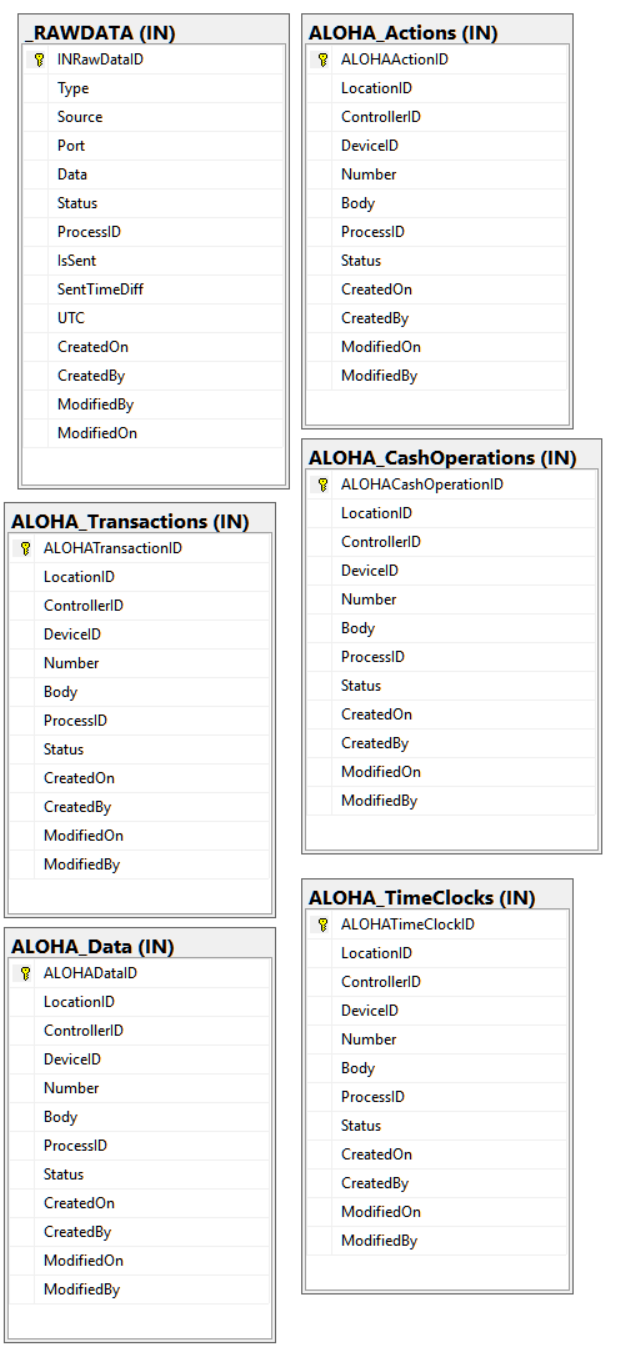
\includegraphics[width=\textwidth]{./img/preparser_database_schema.png}
	\caption{Schemat bazy danych dla modułu wstępnego przetwarzania.}
	\label{fig:preparser_database_schema}
\end{figure}
Moduł właściwego przetwarzania danych.
Schemat bazy danych zawierający niżej wymienione tabele odpowiadające za pracę Parsera (rys. \ref{fig:parser_database_schema}):
\begin{itemize}
	\item Transactions,
	\item TransactionProducts,
	\item TransactionPayments,
	\item TransactionDiscounts,
	\item TransactionReceipts,
	\item TransactioActions.
\end{itemize}
\begin{figure}[t]
	\centering
	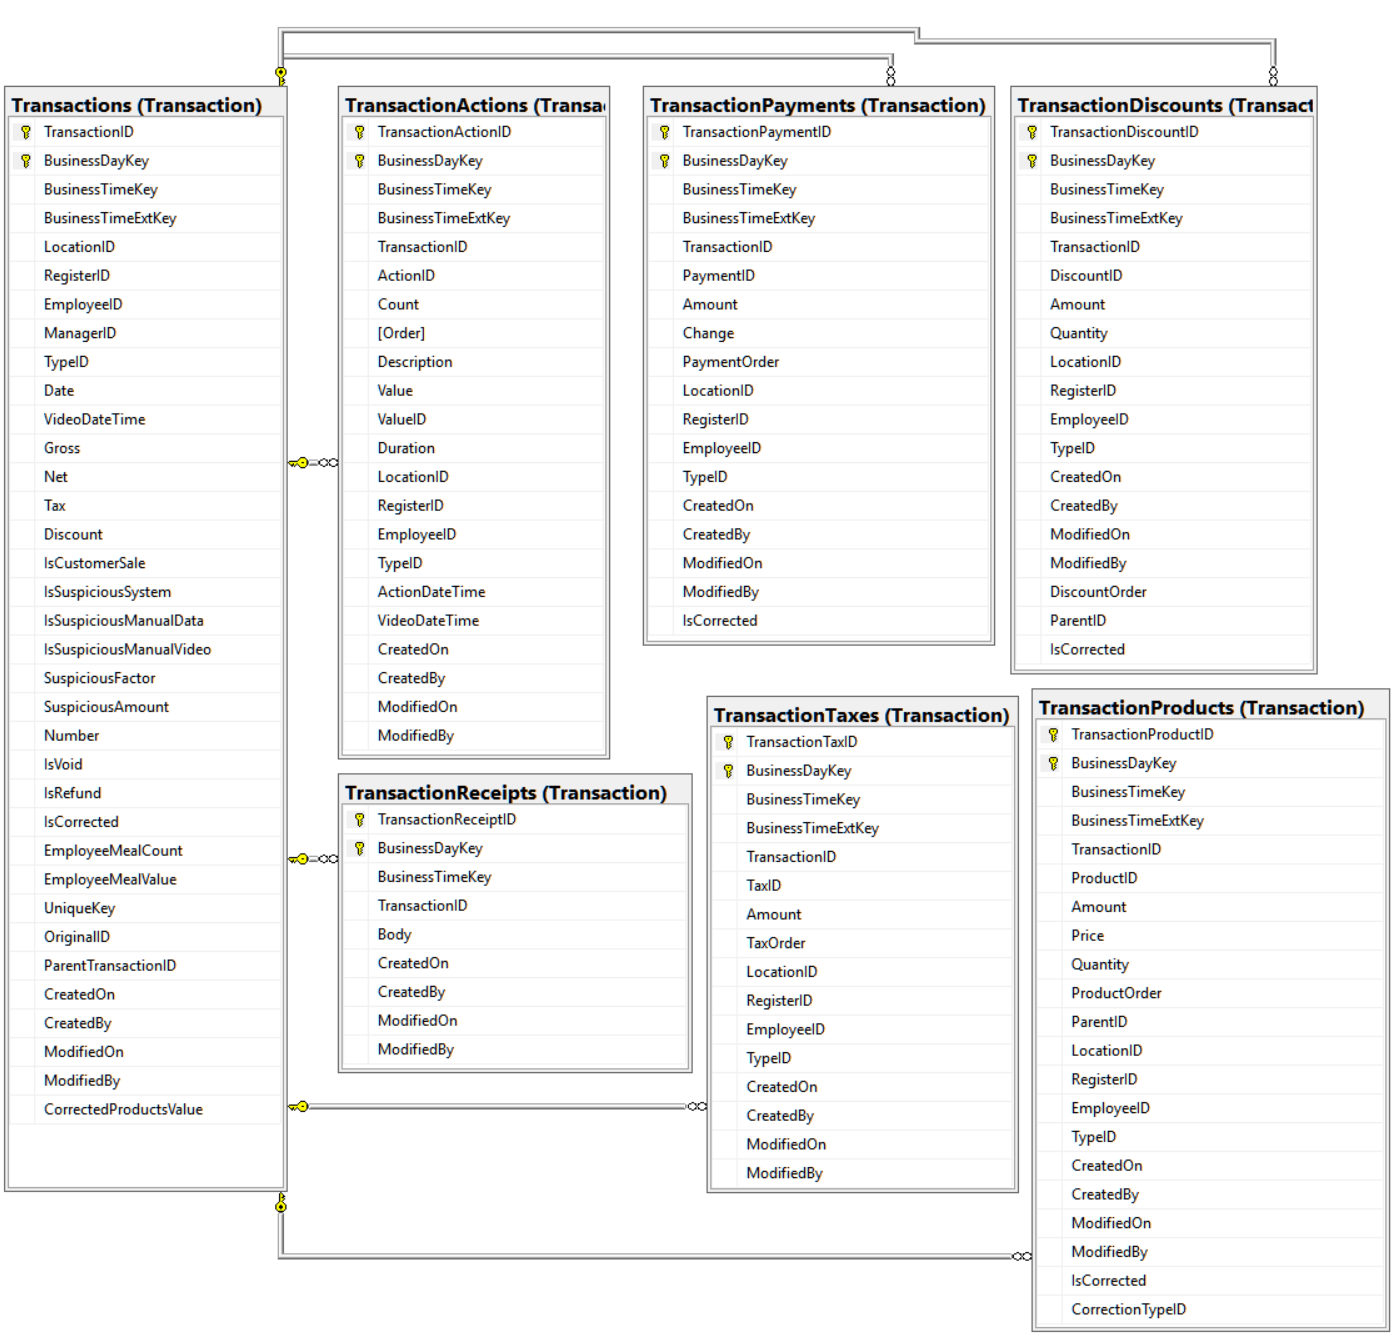
\includegraphics{./img/parser_database_schema.png}
	\caption{Schemat bazy danych dla modułu właściwego przetwarzania.}
	\label{fig:parser_database_schema}
\end{figure} 
\section{Hierarchia klas}
W celu realizacji zadania zostały zaproponowane hierarchie klas dla PreParsera i Parsera, które zostały przedstawione na rys. \ref{fig:preparser_diagram_klas} i  rys. \ref{fig:parser_diagram_klas}. 
\begin{itemize}
	\setlength\itemsep{0.1pt}
	\item Moduł wstępnego przetwarzania danych (rys. \ref{fig:preparser_diagram_klas}),
	\subitem \textbf{PreParser} - jest to główna klasa abstrakcyjna, po której dziedziczą wszystkie PreParsery działające w obrębie systemu 360iQ. Dostarcza ona podstawowych funkcjonalności wspomagających ogólny proces wstępnego przetwarzania danych.
	\subitem \textbf{AlohaPreParser} - klasa dziedzicząca po klasie PreParser i rozbudowująca jej funkcjonalności i rozwiązania specyficzne dla terminali Aloha. Administruje ona podziałem danych wejściowych na odpowiednie typy, dla których później uruchamia specjalne klasy przetwarzające.
	\subitem \textbf{TransactionPreParser} - klasa zaprojektowana w celu wstępnego przetwarzania transakcji.
	\subitem \textbf{TimeClockPreParser} - klasa zaprojektowana w celu wstępnego przetwarzania obecności pracowników.
	\subitem \textbf{CashDropPreParser} - klasa zaprojektowana w celu wstępnego przetwarzania wpłat i wypłat z kasy.
	\item Moduł właściwego przetwarzania danych (rys. \ref{fig:parser_diagram_klas}).
	\subitem \textbf{Parser} - jest to główna klasa abstrakcyjna, po której dziedziczą wszystkie Parsery działające w obrębie systemu 360iQ. Dostarcza ona podstawowych funkcjonalności wspomagających ogólny proces właściwego przetwarzania danych.
	\subitem \textbf{AlohaParser} - klasa dziedzicząca po klasie Parser i dodająca wsparcie dla terminali kasowych Aloha. Odczytuje typy obiektów, które zostały przekazane w formie danych wejściowych i uruchamia specjalne klasy przetwarzające.
	\subitem \textbf{TransactionParser} - klasa zaprojektowana w celu właściwego przetwarzania transakcji.
	\subitem \textbf{TimeClockParser} - klasa zaprojektowana w celu właściwego przetwarzania obecności pracowników.
	\subitem \textbf{CashDropParser} - klasa zaprojektowana w celu właściwego przetwarzania wpłat i wypłat z kasy.
	\subitem \textbf{DataParser} - klasa zaprojektowana w celu właściwego przetwarzania danych dodatkowych.
\end{itemize}
\begin{figure}[t]
	\centering
	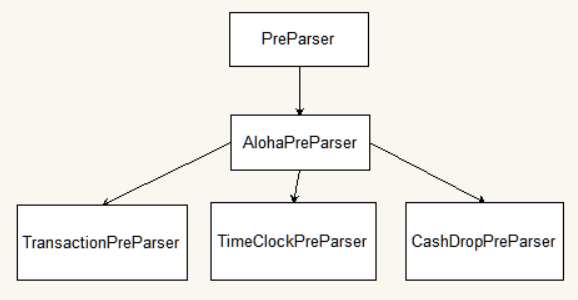
\includegraphics{./img/preparser_diagram_klas.png}
	\caption{Diagram przedstawiający najważniejsze klasy - PreParser.}
	\label{fig:preparser_diagram_klas}
\end{figure}
\begin{figure}[t]
	\centering
	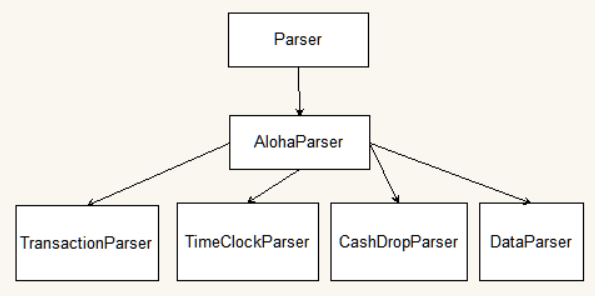
\includegraphics{./img/parser_diagram_klas.png}
	\caption{Diagram przedstawiający najważniejsze klasy - Parser.}
	\label{fig:parser_diagram_klas}
\end{figure}
\section{Szczegółowa analiza danych wejściowych}
Na podstawie przykładowych danych wejściowych przestawionych na rys. \ref{lst:przykladoweZdarzenieAloha2}. Każde zdarzenie w formacie XML zawiera następujące atrybuty:
\begin{itemize}
	\setlength\itemsep{0.1pt}
	\item TerminalID - numer terminala kasowego.
	\item EventTime - czas wystąpienia zdarzenia.
	\item EmployeeID - ID pracownika.
	\item EmployeeName - imię i nazwisko pracownika.
	\item ManagerID - ID managera.
	\item ManagerName - imię i nazwisko managera.
	\item TableID - ID stanowiska, na którym ulokowany jest terminal.
	\item CheckID - numer transakcji.
	\item TransactionTypeID - ID typu zdarzenia.
	\item TransactionType - nazwa typu zdarzenia.
	\item Description - opis zdarzenia.
	\item Amount - wartość pieniężna związana ze zdarzeniem.
	\item Quantity - ilość sztuk (w przypadku produktów i płatności).
	\item Sender - adres IP urządzenia wysyłającego.
	\item ReceivedOn - data otrzymania zdarzenia po stronie kontrolera.
\end{itemize}
\begin{figure}[t]
	\begin{lstlisting}[frame=single, breaklines=true, numbers=none]
	<SpyMessage 
		TerminalID="4" 
		EventTime="23:59:57" 
		EmployeeID="94205" 
		EmployeeName="AHMET B?RL?K" 
		ManagerID="0" 
		ManagerName="" 
		TableID="4194420" 
		CheckID="40116" 
		TransactionTypeID="59" 
		TransactionType="TOTAL" 
		Description="" 
		Amount="18.75" 
		Quantity="0" 
		Sender="192.168.100.4" 
		ReceivedOn="2017.11.30 00:00:08.204" 
	/>
	\end{lstlisting}
	\caption{Przykładowe zdarzenie - dane wejściowe Aloha.}
	\label{lst:przykladoweZdarzenieAloha2}
\end{figure}
\section{Algorytmy}
W systemie wykorzystane zostały następujące algorytmy przetwarzające i~rozszerzające dane wejściowe w formacie XML:
\begin{itemize}
	\item Dodawanie brakujących przedmiotów będących częścią promocji do transakcji (rys.  \ref{lst:brakujaceProdukty}).
	\item Rozszerzanie zdarzenia XML o rozszerzone nazwy przedmiotów (rys. \ref{lst:rozszerzanieXML}).
\end{itemize}
\subsection{Dodawanie brakujących przedmiotów będących częścią promocji do transakcji}
Raz w ciągu dnia, otrzymywana jest wiadomość zawierająca PromotionsXML. Za każdym razem, gdy taka informacja jest odbierana, zapisana zostaje do pliku lub aktualizowana, jeśli już istnieje. PreParser zawiera również obiekt, który przechowuje dane pochodzące ze słownika PromotionsXML. Wspomniana wiadomość jest konwertowana na instancję klasy PromotionBundle, która przechowuje informacje o promocjach i elementach w niej zawartych. Metoda bezpośrednio zaangażowana w przetwarzanie promocji nazywa się ProcessAddPromo. Zapewnia funkcjonalność, która wykrywa, czy nastąpiła zmiana promocji i wstawia produkty, których brakuje. To, co dokładnie dzieje się w wykrywaniu algorytmów promocji, można podsumować w prostych krokach:
\begin{itemize}
	\item Przechowywana jest historia przetworzonych zdarzeń, co pozwala algorytmowi powrócić do przeszłych akcji, aby wykryć pożądany schemat,
	\item Szukany jest zestaw 2 instrukcji - ADD\_ITEM, CANCEL\_ITEM - (jest to wartość minimum - zostaje ona zwiększona, jeśli wykryte są zdarzenia, których zawartość pola TransactionType zaczyna się od 6 lub 7), które poprzedzały bieżące zdarzenie,
	\item Jeśli znaleziony zostanie odpowiedni zestaw zdarzeń, który jest rozpoznawany jako zmiana promocji to dodawane lub usuwane są odpowiednie wydarzenia na podstawie wyników wyszukiwania odpowiednich schematów zdarzeń.
\end{itemize}
\begin{figure}[t]
	\begin{lstlisting}[frame=single, breaklines=true]
	private void ProcessAddPromo(XElement action, XElement lastAction, List<SpyMessage> actions,
	List<PromotionBundle> promotionBundles, List<string> warningMessages, List<SpyMessage> result)
	{
		var listOfActions = actions.Select(x => x.Body).ToList();
		var lastActionTransactionType = lastAction?.Attribute("TransactionType")?.Value ?? string.Empty;
		//Warunkiem rozpoczecia pracy algorytmu jest zidentyfikowanie typu obecnie przetwarzanego zdarzenia jako DELETE_PROMO
		if (lastActionTransactionType == "DELETE_PROMO")
			{
				var actionsOffset = 2;
				var cancelItemActionAppeared = false;
				var addItemActionAppeared = false;
	
				//Sprawdza czy w obrebie 2 zdarzen, ktore wystapily przed obecnie analizowanym zdarzeniem wystapily zdarzenia typu ADD lub CANCEL
				CheckIfAddOrCancelActionAppeared(listOfActions, lastAction, actionsOffset, cancelItemActionAppeared, addItemActionAppeared);
				if (addItemActionAppeared)
				{
					//Wystapilo zdarzenie ADD, wiec nie ma koniecznosci dodania nowych przedmiotow do transakcji
					IsPromoChanged = true;
					AreItemsAlreadyAdded = true;
				}	
				if (!AreItemsAlreadyAdded)
				{
				//Odczyt nazwy promocji w celu znalezienia jej produktow skladowych ze slownika promotionBundles    
				var promoName = action?.Attribute("Description")?.Value ?? string.Empty;
				var bundle =
				promotionBundles.FirstOrDefault(x => x.PromotionName.ToUpperInvariant() ==
				promoName.ToUpperInvariant());
				//Obsluga promocji typu: 2 za 1$
				var itemsMultiplier = 1;
				if (promoName.StartsWith("2 for"))
				{
				itemsMultiplier = 2;
				}
	
				//Dodanie brakujacych zdarzen opisujacych dodanie wymaganych przedmiotow do transakcji
				AddMissingItemsXML(bundle, itemsMultiplier, actions, result);
				}
				
			//Ustawienie flagi na false w celu obslugi kolejnego przebiegu algorytmu dla nastepnych danych
			AreItemsAlreadyAdded = false;
		}
	}
	\end{lstlisting}
	\caption{Dodawanie brakujących przedmiotów będących częścią promocji do transakcji}
	\label{lst:brakujaceProdukty}
\end{figure}
\subsection{Rozszerzanie zdarzenia XML o rozszerzone nazwy przedmiotów i wartości podatków}
Raz w ciągu dnia, pojawia się komunikat zawierający ItemCategoryXML. Dostarcza on rozszerzonych informacji o przedmiotach i ich kategoriach. W~Aloha ten sam przedmiot może być nazwany z wykorzystaniem różnych formatów.
Biorąc to pod uwagę, opracowano funkcjonalność rozszerzającą przychodzące zdarzenie XML z danych wejściowych.
Dodaje ona nowe atrybuty do istniejącego pliku XML z wymienionymi wyżej nazwami elementów. Nazwa przedmiotu jest identyfikowana za pomocą tego algorytmu:
\begin{itemize}
	\item Nazwa przedmiotu (lub jej odmiany) jest wyodrębniona z atrybutu Description,
	\item Uzyskana nazwa porównywana jest z nazwami produktu pochodzącymi z~ItemCategoryXML,
	\item Gdy tylko znaleziona zostanie pasująca nazwa, znajdowane są wszystkie jej odmiany i rozszerzana jest wiadomość XML o dodatkowe pola z odpowiednimi wartościami,
	\item Od tego momentu zdarzenie zawiera wszystkie potrzebne informacje o~przedmiocie, które mogą być wykorzystane podczas dalszego przetwarzania.
\end{itemize}
Metoda implementująca tę funkcjonalność to: ExtendMessegeWithAdditionalItemInfo.
Słownik ItemCategoryXML jest przechowywany zarówno na dysku, jak i jako obiekt XElement po stronie serwisu. Jest aktualizowany za każdym razem, gdy przychodzi nowa wiadomość z nową wersją ItemCateogryXML.
\begin{figure}[t]
	\begin{lstlisting}[frame=single, breaklines=true]
	private void ExtendMessegeWithAdditionalItemInfo(XElement action, XElement itemCategoryXML, List<TaxInformation> taxInformations, List<PromotionBundle> promotionBundles)
	{
		//Pobranie nazwy przedmiotu z atrybutu XML
		var itemName = action?.Attribute("Description")?.Value ?? string.Empty;
		//Jezeli slownik jest rozny od NULL to uruchamiamy algorytm
		if (itemCategoryXML != null)
		{
			//Lista przedmiotow ze slownika
			var itemNodes = itemCategoryXML.Elements();
			//Dodanie do obecnej akcji typu ADD/CANCEL/VOID rozszerzonych nazw z pustymi wartosciami
			AddNewAttributesWithEmptyValues(action);
			
			//Ustawianie wartosci rozszerzonych nazw dla przetwarzanej akcji na podstawie zawartosci kolekcji itemNodes, 
			//ktora pochodzi ze slownika z lista produktow, dostarczona przez uzytkownika
			foreach (var item in itemNodes)
			{
				var itemShortName = item?.Attribute("ItemShortName")?.Value ?? string.Empty;
				var itemLongName = item?.Attribute("ItemLongName")?.Value ?? string.Empty;
				var itemLongName2 = item?.Attribute("ItemLongName2")?.Value ?? string.Empty;
				var itemChitName = item?.Attribute("ItemChitName")?.Value ?? string.Empty;
				var itemNameAttr = item?.Attribute("ItemName")?.Value ?? string.Empty;
				//Sprawdzanie czy ktoras z nazw przechowywanych w slowniku pokrywa sie z otrzymana w zdarzeniu.
				//Jesli tak to rozszerzamy zdarzenie o dodatkowe nazwy.	
				if (!string.IsNullOrEmpty(itemShortName) && itemShortName == itemName
				|| !string.IsNullOrEmpty(itemLongName) && itemLongName == itemName
				|| !string.IsNullOrEmpty(itemLongName2) && itemLongName2 == itemName
				|| !string.IsNullOrEmpty(itemChitName) && itemChitName == itemName
				|| !string.IsNullOrEmpty(itemNameAttr) && itemNameAttr == itemName)
				{
					action.SetAttributeValue("ItemId", item?.Attribute("ItemId")?.Value ?? string.Empty);
					action.SetAttributeValue("ItemShortName", itemShortName);
					action.SetAttributeValue("ItemLongName", itemLongName);
					action.SetAttributeValue("ItemLongName2", itemLongName2);
					action.SetAttributeValue("ItemChitName", itemChitName);
					action.SetAttributeValue("ItemName", itemNameAttr);
				}
			}
		}
	}
	\end{lstlisting}
	\caption{Rozszerzanie zdarzenia XML o rozszerzone nazwy przedmiotów.}
	\label{lst:rozszerzanieXML}
\end{figure}

\chapter{Testowanie i uruchamianie}
\label{rozdzial6}
W niniejszym rozdziale zostaną opisane przeprowadzone testy zarówno dla moduł wstępnego przetwarzania danych jak i części odpowiedzialnej za właściwe przetwarzanie informacji. Dane testowe zostały zaimportowane w formie kopii zapasowej bazy danych z lokalizacji, na której codziennie działa opisane w tej pracy rozwiązanie. Testowane przypadki obejmują dane zawarte w zrzucie z bazy danych (03-11-2017) z lokalizacji położonej na terenie Stanów Zjednoczonych. Z racji faktu przeprowadzenia znacznej ilości testów oraz analizy przypadków testowych, autor niniejszej pracy ograniczył się do umieszczenia tylko tych najbardziej podstawowych, ponieważ całościowy opis i analiza testowanych przypadków nie był możliwy z racji zbyt ich dużego stopnia skomplikowania oraz obszerności. 
\section {PreParser}
Tabela \ref{tab:testy_preparser} przedstawia wyniki procedury testowej modułu wstępnego przetwarzania.
Dane wejściowe zgromadzone są w tabeli \_RAWDATA i wyniki ich analizy powinny zostać umieszczone w tabelach: Aloha\_Transactions, Aloha\_TimeClocks, Aloha\_CashOperations. Całość tabel znajduję się bazie EZ360Communication. 
\begin{table}
	\centering
	\caption{Testy modułu wstępnego przetwarzania danych.}
	\begin{tabular}{|c|c|c|c|}
		\hline
		\thead{Testowany przypadek} & \thead{Dane wejściowe} & \thead{Dane wyjściowe} & \thead{Wynik} \\
		\hline
		\makecell{Przetwarzanie całości\\danych wejściowych\\z testowanej paczki.} & \makecell{Zawartość tabeli \_RAWDATA. \\Ilość zdarzeń \\do przetworzenia - 78490}  &  \makecell{Liczba przetworzonych \\danych: \\Transactions-3700,\\TimeClocks-232,\\CashOperations-34} & \makecell{Poprawny}\\
		\hline
		\makecell{Przypadek pustej tabeli\\ z~danymi wejściowymi.} & \makecell{Zawartość tabeli \_RAWDATA. \\Ilość zdarzeń \\do przetworzenia -~ 0}  & \makecell{Brak danych\\ do przetworzenia. \\PreParser oczekuje \\na przyjście\\ nowych danych\\ do przetwarzania.} & \makecell{Poprawny}\\
		\hline
		\makecell{Przypadek tabeli\\z danymi\\wejściowymi zawierającymi\\jedną niepełną\\transakcję.} & \makecell{Zawartość tabeli \_RAWDATA.\\Ilość zdarzeń\\do przetworzenia -~ 9.\\Brak zdarzenia\\kończącego transakcje.}  & \makecell{Dane zostają\\przetworzone,\\jednakże transakcja\\nie zostaje wysłana,\\ponieważ PreParser\\czeka na przyjście\\zdarzenia kończącego\\transakcje.} & \makecell{Poprawny}\\
		\hline
		\makecell{Przypadek tabeli\\z~danymi wejściowymi\\zawierającymi jedną\\pełną transakcję.} & \makecell{Zawartość tabeli \_RAWDATA. \\Ilość zdarzeń\\do przetworzenia -~ 10.\\Występuje zdarzenie\\ kończące transakcje.}  & \makecell{Dane zostają\\przetworzone,\\transakcja zostaje\\wysłana.} & \makecell{Poprawny}\\
		\hline 
	\end{tabular}
	\label{tab:testy_preparser}
\end{table}
\section {Parser}
Tabela \ref{tab:testy_parser} przedstawia wyniki procedury testowej modułu właściwego przetwarzania.
Dane wejściowe zgromadzone są w tabelach: Aloha\_Transactions, Aloha\_TimeClocks, Aloha\_CashOperations i wyniki ich analizy powinny zostać umieszczone w tabelach: Transaction.Transactions, Transaction.Taxes, Transaction.Receipts, Transaction.Products, Transaction.Payments, Transaction.Discounts (EZ360Sales) oraz Employee.Employees, Employee.EmployeeAttendances (EZ360Labor). 
\begin{table}
	\centering
	\caption{Testy modułu właściwego przetwarzania danych.}
	\begin{tabular}{|c|c|c|c|}
		\hline
		\thead{Testowany przypadek} & \thead{Dane wejściowe} & \thead{Dane wyjściowe} & \thead{Wynik} \\
		\hline
		\makecell{Przetwarzanie transakcji} & \makecell{Zawartość tabeli\\Aloha\_Transactions.\\Ilość zdarzeń\\do przetworzenia- 3700}  &  \makecell{Dodano 3700\\nowych transakcji\\do systemu.} & \makecell{Poprawny}\\
		\hline
		\makecell{Procesowanie\\wpłat/wypłat\\z kasy} & \makecell{Zawartość tabeli\\Aloha\_CashOperations.\\Ilość zdarzeń\\do przetworzenia - 34}  &  \makecell{Dodano 34\\nowych wpłat/wypłat\\do systemu.}  & \makecell{Poprawny}\\
		\hline
		\makecell{Procesowanie\\wpłat/wypłat\\z kasy} & \makecell{Zawartość tabeli\\Aloha\_TimeClocks.\\Ilość zdarzeń\\do przetworzenia - 232}  & \makecell{Dodano 232\\nowych informacji\\o obecnościach\\pracowników\\do systemu.} & \makecell{Poprawny}\\
		\hline
		\makecell{Brak danych\\do przetworzenia} & \makecell{Pusta tabela\\Aloha\_Transactions.} & \makecell{Parser czeka\\na nadejście\\danych do\\przetworzenia.} & \makecell{Poprawny}\\
		\hline 
		\makecell{Błędne dane\\wejściowe} & \makecell{Tabela\\Aloha\_Transactions\\z~transakcjami\\zawierającymi błędne\\XML-e.} & \makecell{Parser oznacza\\nieprawidłowe dane\\odpowiednim statusem\\i kontynuuje pracę.} & \makecell{Poprawny}\\
		\hline 
	\end{tabular}
	\label{tab:testy_parser}
\end{table}
\chapter{Uwagi o przebiegu i~wynikach prac oraz podsumowanie}
\label{rozdzial7}
\section {Stopień realizacji zagadnienia}
Opisywane w poprzednich rozdziałach zagadnienie zostało zrealizowane w~stopniu całkowitym. Aplikacja przeszła pomyślnie proces projektowania, tworzenia oraz testów. Jest ona wdrożona jako część systemu 360iQ udostępnianego przez firmę EZUniverse i widnieje w nim pod nazwami AlohaPreParser oraz AlohaParser. Oprogramowanie stabilnie działa na dużej liczbie kontrolerów i dostarcza wysoce wiarygodne dane, mogące być analizowane przez użytkownika systemu.
\section{Napotkane problemy}
Głównymi problemami, które generuje terminal kasowy Aloha, są rozdrobnione i niespójne dane. Każda transakcja dostarczana jest jako seria zdarzeń, które niekoniecznie zostają wysyłane do kontrolera w należytym porządku. Wymagało to implementacji funkcjonalności łączącej zdarzenia w grupy, które można opisywać jako transakcje lub inne zdarzenia zachodzące na kasie. Dodatkowymi problemami były nieścisłości związane z produktami zawartymi w promocjach oraz wiele nazw, które opisywały ten sam przedmiot. Rozwiązano te problemy wykorzystując opisane wcześniej w niniejszej pracy algorytmy rozszerzające i~modyfikujące dane.
\section{Dalszy rozwój}
Z racji faktu ciągłej pracy systemu, konieczne jest jego stałe wspieranie oraz aktualizowanie. Rozwiązywane są również zgłaszane przez klienta usterki i~błędy w przetwarzaniu danych. Konieczność ciągłej rozbudowy aplikacji wynika z wdrażania systemu na coraz większą ilość lokalizacji co wymaga specjalnych poprawek lub optymalizacji wynikających z uwarunkowań regionalnych.
\section{Podsumowanie}
Realizowanym zagadaniem w niniejszej pracy było stworzenie systemu przetwarzania danych z terminali kas sklepowych Aloha, który ma być częścią systemu 360iQ zaprojektowanego przez firmę EZUniverse. Miał on na celu umożliwienie właścicielowi sklepu analizy danych sprzedażowych oraz wpłat i wypłat z kas sklepowych. W tym celu zaimplementowano moduły wstępnego (PreParser) oraz właściwego (Parser) przetwarzania danych.
W niniejszej pracy opisano proces realizacji zagadnienia, którym autor zajmuję się regularnie w ramach pracy zawodowej. Wiedza zdobyta podczas pracy z tym typem danych (tj. danych generowanych przez terminale kas sklepowych) oraz urządzeń, pozwoliła zbudować od samych podstaw własny moduł realizujący kompleksowe przetwarzanie danych. Opracowane zostały specjalne algorytmy przetwarzające dane wejściowe (rozdział \ref{rozdzial5}), które weszły w skład funkcjonalności dostarczanej przez PreParser, który zapewnia możliwości pozwalające na wstępną obróbkę i przygotowanie danych do dalszego etapu przetwarzania. Zaimplementowano również szereg funkcjonalności tworzących moduł Parsera, składają się one na przetwarzanie: transakcji, wpłat/wypłat z kasy, obecności pracowników. Pod koniec procesu przetwarzania danych wejściowych moduł właściwej analizy danych umieszcza je w wynikowej bazie danych. Aplikacja przeszła szereg wymagających testów sprawdzających jakość przetwarzanych danych oraz ich poprawność. Autor postanowił wykorzystać wiedzę i doświadczenie zdobyte podczas pracy zawodowej oraz studiów, by stworzyć system mający być częścią oprogramowania 360iQ dostarczanego przez firmę EZUniverse Inc. Dzięki regularnej pracy nad zagadnieniem podczas wykonywania obowiązków zawodowych oprogramowanie zostało wdrożone w sklepach na całym świecie (największa ilość wspieranych sklepów znajduję się na terenie Stanów Zjednoczonych) i~jest ono na bieżąco monitorowane oraz rozwijane przez autora w związku z pełnieniem obowiązków zawodowych.
\bibliographystyle{plunsrt}
\bibliography{bibliografia}
\end{document}
